\section{Coaching Stage}
The coaching stage takes in high-level user instructions and
interprets them by revising the task objective or adding
constraints. We introduce ``control rigs'', as an intermediate layer
between high-level instructions and low-level control variables. A
control rig, predefined by our framework, is a function of a set of
low-level control variables. It allows for more coordinated control of
the low-level variables and provides more intuitive mapping to
high-level instructions. The main advantage of using control
rigs is that it reduces the optimization time significantly by
suggesting the most effective directions to optimize. Although a
control rig needs to be manually defined, it can be shared by
different instructions or repurposed for new motor tasks.

\subsection{Instructions}
\label{sec:parkour_instructions}

Although coaching strategies and styles vary widely, the basic
instructions commonly used to break down a complex movement are
surprisingly consistent. Most instructions provide a numerical or
categorical correction to improve a particular part of the body. For example,
``Lower the center of mass more'' or ``raise your arms to 45 degrees''.  
From observing Parkour training sessions and tutorials, we
define a set of coaching instructions in Table \ref{tab:parkour_map}.

\subsection{Control Rigs}
A control rig $r$ is a pre-defined function of a set of low-level PD
or Jacobian Transpose controllers.  A PD controller tracks
the target joint angle based on the feedback rule: $\tau = k_s
(\hat{\theta} -\theta) - k_d (\dot{\theta})$, where $k_s$ and $k_d$
are the gain and the damping coefficient of the joint and
$\hat{\theta}$ is the desired value for the joint angle. A Jacobian
Transpose controller computes the required joint torques to produce
the desired ``virtual force'', $\vc{f}_v$, at a point $\vc{x}$,
using the Jacobian Transpose mapping: $\tau =
\vc{J}^T(\vc{x})\vc{f}_v$, where $\vc{J}(\vc{x})$ is the Jacobian
matrix at $\vc{x}$. These two types of low level controllers, when
combined properly, can effectively control the pose and global motion
of the character. A control rig, $\tau = r(\vc{q}_t, \vc{p})$, takes
in the current state $\vc{q}_t$ and the rig parameters $\vc{p}$ to
produce torques which are added to the total torques applied to the
character.

We keep a set of active control rigs, $\mathcal{R} = \{r_1, ..., r_m\}$, during
training. As the user provides more instructions, more control rigs
are included to the active set. With optimized parameters $\mathcal{P} = \{\vc{p}_1,
..., \vc{p}_m\}$, we obtain an improved controller $g_R$.
\begin{equation}
  \begin{aligned}
    g_{\mathcal{R}}(\vc{q}, \mathcal{P}) = g(\vc{q}) + \sum_{i=1}^m r_i(\vc{q}, \vc{p}_i)
  \end{aligned}
\end{equation} 

In this paper, we designed five control rigs from common instructions
used for learning gymnastics and Parkour. Each control rig,
$r_i$, has a set of arguments determined by the instruction from which
$r_i$ is created, and a set of rig parameters which are optimized
during the practicing stage (Table \ref{tab:parkour_rigs}).

\begin{enumerate}
\item{TargetJoints rig consists of the PD
      controllers on a set of joints specified by the instruction. The
      rig parameters are defined as the target joint angles of the PD controllers.}
\item{IKPose rig solves for the joint angles to meet a desired
      relative position of two bodies specified by the instruction. The
      solved joint angles are then used as the target angles for a set
      of PD controllers. }
\item{Stiffness rig adjusts the gains of the PD
  controllers on a set of joints specified by the instruction. The rig
  parameters are defined as the gains. }
\item{VirtualForce rig consists of a Jacobian Transpose
  controller which computes required torques to produce a virtual
  force at the center of mass of a body link specified by the instruction. The rig parameter is
  defined as the desired virtual force}
\item{FeedbackVirtualForce rig consists of a Jacobian
      Transpose controller on a body link specified by the
      instruction. Instead of treating the desired virtual force as a
      rig parameter, it is computed using the feedback rule:
      $f_v = k_s(\hat{\vc{C}} - \vc{C}) - k_d\vc{\dot{C}}$, where
      $\vc{C}$ and $\hat{\vc{C}}$ are the center of mass of the whole body and its
      desired position. Intuitively, this rig computes the torques that generate
      a virtual force to bring the center of mass closer to the desired position.}
\end{enumerate} 

We show that these five control rigs are sufficient to
generate the motor skills demonstrated in the result section.


\begin{table}
  \center
  \scriptsize
  \caption{Control rigs.     \hspace*{\fill} }
  \begin{minipage}{\textwidth}
  \begin{tabular}{ | l | p{5.8cm} | p{3.0cm} |}
    \hline
    \textbf{Rig Type $<$Arguments$>$}& \textbf{Description} & \textbf{Rig Parameters} \\ \hline
    TargetJoints $<$joint a, $\cdots>$ & Command a set of joints to achieve desired angles
    simultaneously. & Desired joint angles \\ \hline
    IKPose $<$body a, body b$>$ & Compute a target pose to meet the
    desired relative position
    between body a and body b. Command joints to achieve the
    target pose. & Desired distance or desired angles \\ \hline
    Stiffness $<$ joint a, $\cdots>$ & Command a set of joints with desired stiffness. & Gains \\ \hline
    VirtualForce $<$body a$>$ & Apply torques which produce the
    desired virtual force at the center of mass of body a. &
    \footnote{$f_u$ is  in the direction of C - S. $f_v$ is orthogonal to $f_u$
      and parallel to the contacting surface.}
    Desired virtual force in end-effector frame
    %% \footnote{$f_u$ is  in the direction of C - S. $f_v$ is orthogonal to $f_u$ and parallel to the contacting surface.} 
    \\ \hline
    FeedbackVirtualForce $<$body a, 
    $\hat{\vc{C}}$ $>$ 
    & 
    \footnote{We use the following feedback rule on the center of mass
      of the whole body: $f_v = k_s(\hat{\vc{C}} - \vc{C}) -
      k_d\vc{\dot{C}}$, where $k_s = 300$ and $k_d = 6$.}
    Apply torques which produce the virtual force at the
    cetner of mass of body a. The virtual force is computed by a
    feedback rule.  & -
    \\ \hline 
  \end{tabular}
  \label{tab:parkour_rigs}
  \end{minipage}
\end{table}


\begin{table}[t]
  \center
  \scriptsize
  \caption{
    Interpretation of instructions. Each instruction is
    associated with a control rig, an objective
    term and/or a contraint.
    $\vc{q}_f$, $\vc{q}^{prev}_f$ : the final state of the current motion
    and the previous motion.
    $\vc{C}, \vc{S}, \vc{P},\vc{L}$ : the center of mass, center of pressure, 
    linear momentum, and angular momentum.  
    $\vc{pos}_{limb}$, $\vc{rot}_{limb}$ : the limb position and orientation. 
    $q_{joint}, ks_{joint}$ : the joint angle and stiffness.
    \hspace*{\fill}
  } 
  \begin{minipage}{\textwidth}
    \begin{tabular}{ | p{3.7cm} | p{3.7cm} | c |}
      \hline
      \textbf{Instruction }
      %% & \revthree{Example} 
      & \textbf{Introduced control rig }
      & \textbf{Introduced objective / constraint} \\ \hline

      FLEX$|$EXTEND joint BY $\theta$ 
      %% & \revthree{FLEX elbows BY $60^{\circ}$}
      & TargetJoints$<$joint$>$
      & $ \| q_{joint} (\vc{q}_f) - \theta \|$ \\ \hline

      MOVE 
      \footnote{We used a dictionary to translate the dir keyward into
        direction vector d. For instance, if the dir keyword is ``upward'', $d
        = (0, 1, 0)^T$. }
      direction BY $\delta$
      %% & \revthree{MOVE downward BY $0.2m$}
      & IKPose$<$
      \footnote{``contact'' indicates the body parts in contact}
      contact, root$>$
      &  
      \footnote{We project $\vc{C}(\vc{q})$ in the desired direction, $\vc{d}$,
        specified in the instruction.} 
      $ \|\vc{C}(\vc{q}_f) \cdot \vc{d} - (\vc{C}(\vc{q}^{prev}_f) \cdot \vc{d} + \delta)\|$ \\ \hline

      TRANSLATE limb direction BY $\delta$
      %% & \revthree{TRANSLATE hands forward BY $0.5m$}
      & IKPose$<$root, limb$>$
      & $ \|\vc{pos}_{limb}(\vc{q}_f) \cdot \vc{d} - (\vc{pos}_{limb}(\vc{q}^{prev}_f) \cdot \vc{d} + \delta)\|$ \\ \hline

      ROTATE limb direction BY $\delta$
      %% & \revthree{ROTATE spine x-axis BY $30^{\circ}$}
      & IKPose$<$root, limb$>$
      & $ \|\vc{rot}_{limb}(\vc{q}_f) \cdot \vc{d} - (\vc{rot}_{limb}(\vc{q}^{prev}_f) \cdot \vc{d} + \delta)\|$ \\ \hline

      SPEED NEAR $\hat{\dot{\vc{C}}}$ 
      %% & \revthree{SPEED NEAR $[1.2, 2.4, 0.0]^Tm/s$}
      & VirtualForce$<$contact$>$
      %% & $ \|\dot{\vc{C}}(\vc{q}_f) - \hat{\dot{\vc{C}}}(\vc{q}_f)\|$ \\ \hline
      & $ \|\dot{\vc{C}}(\vc{q}_f) - \hat{\dot{\vc{C}}}\|$ \\ \hline

      SPEEDUP/ SLOWDOWN $\gamma$ \% 
      %% & \revthree{SPEEDUP $150$ \%}
      & VirtualForce$<$contact$>$
      & $ \|\vc{P}(\vc{q}_f) - (\vc{P}(\vc{q}^{prev}_f) * \gamma) \|$ \\ \hline

      TURNFASTER/ TURNSLOWER $\gamma$ \% 
      %% & \revthree{TURNSLOWER 70\%}
      & VirtualForce$<$contact$>$
      & $ \|\vc{L}(\vc{q}_f) - (\vc{L}(\vc{q}^{prev}_f) * \gamma) \|$ \\ \hline

      BALANCE 
      %% & \revthree{BALANCE}
      & FeedbackVirtualForce$<$ contact, $\hat{\vc{C}}_{bal}$ $>$
      & $ \|\dot{\vc{C}}(\vc{q}_f)\|$ \\ \hline

      RELAX$|$STIFFEN joint BY $\gamma$ \% 
      %% & \revthree{RELAX shoudlers BY 40\%}
      & Stiffness$<$joint$>$
      & $ \|ks_{joint} (\vc{q}_f)- (ks_{joint}(\vc{q}^{prev}_f) \cdot \gamma) \|$ \\ \hline

      PUSH/PULL limb AGAINST surface 
      %% & \revthree{PUSH feet AGAINST wall}
      & VirtualForce$<$limb$>$
      & - \\ \hline

      PLACE body$|$C$|$S NEAR body$|$C$|$S$|$constant 
      %% & \revthree{PLACE hands NEAR head}
      & - 
      & $\|\vc{pos}_{body|C|S}(\vc{q}_f) - \vc{pos}_{body|C|S|constant}(\vc{q}_f)\|$ 
      \\ \hline

      \footnote{The last instruction creates a constraint, instead of an objective function. }
      body$|$C$|$S IN RELATION TO body$|$C$|$S$|$constant
      %% & \revthree{head IN FRONT OF root}
      & - 
      &  relation(body$|$C$|$S, body$|$C$|$S$|$constant) \\ \hline
    \end{tabular}

    \label{tab:parkour_map}
  \end{minipage}
\end{table}


\subsection{Instruction Interpreter}
The instruction interpreter translates a human-readable instruction into two
possible actions: modifying the task objective or adding constraints for
the optimization problem. In addition, if these actions involve
new control rigs, the instruction interpreter will add them to the
optimization domain. We define a set of simple rules that map the
instructions to the control rigs. Please see details in Table \ref{tab:parkour_map}.

\begin{figure}[tb]
\center
  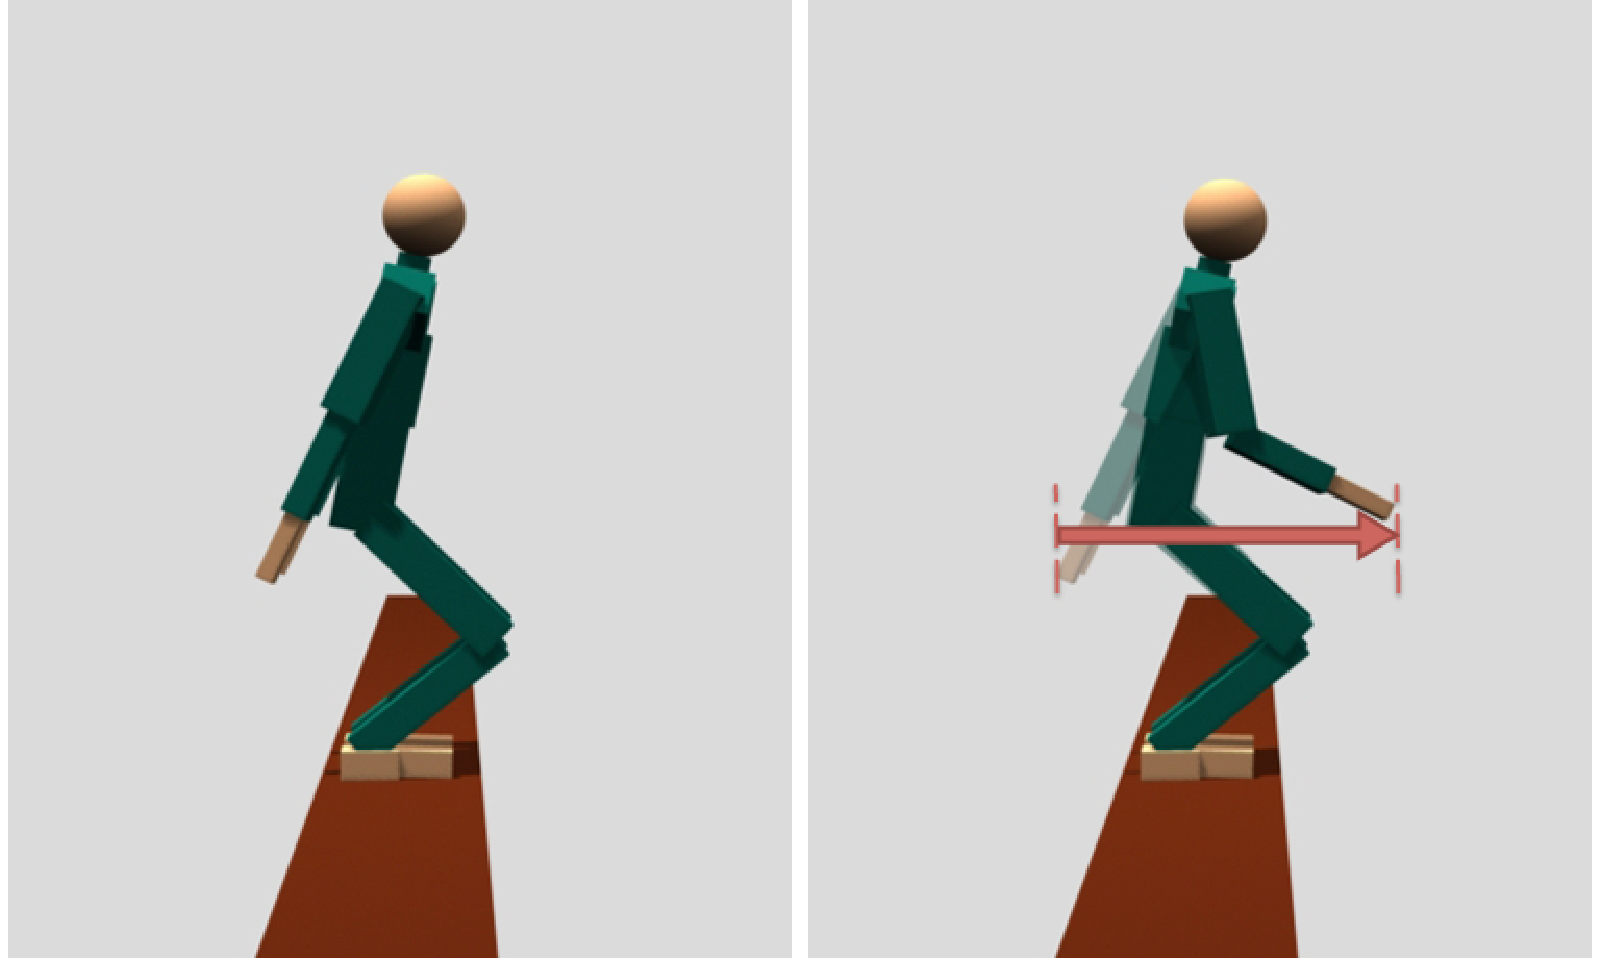
\includegraphics[width=3.0in]{images/instruction_demo}
  \caption{
    The user can adjust the positions of hands by giving an instruction
    ``TRANSLATE hands forward BY $0.5m$''.
    The instruction will add an IKPose rig for arms 
    and modify the desired position of hands by $0.5m$ in the forward direction.
  }
  \label{fig:parkour_instruction_demo}
\end{figure}


\myparagraph{The task objective}
The task objective is evaluated at the final state of the motion by an objective
function
%% \updated{which measures the difference between the current state $h_i$
%% the desired physical value $\hat{h}_i$}
.
\begin{equation}
  f(\mathcal{P}) = \sum_{i=1}^n\|h_i(s(\vc{q}_0, g_{\mathcal{R}}) - \hat{h}_i\|
\label{eq:parkour_costfunc}
\end{equation}

When the user specifies an instruction from \tabref{parkour_map} 
(except for the last instruction, which will be explained in the next paragraph), a new term, $\|h_i(\vc{q}_f) - \hat{h}_i\|$, 
will be added to the objective function. 
$h_i$ is a function that evaluates a quantity derived from the final state. $\hat{h}_i$ is the desired value for
that quantity. 
For example, to interpret the instruction 
``TRANSLATE hands forward BY $0.5m$'' (\figref{parkour_instruction_demo}), 
the keyword ``forward'' is first
mapped to the predefined direction $\vc{d}=[1,0,0]^T$.
Then $h_i(\vc{q}_f)$ is defined as the average position of the hands
in the forward direction $(\vc{pos}_{hands}(\vc{q}_f) \cdot \vc{d})$.
Finally, the desired value $\hat{h}_i$ is computed by adding $0.5m$
to the previous average position of the hands in the forward direction
($\vc{pos}_{hands}(\vc{q}^{prev}_f) \cdot \vc{d} + 0.5$).

Although we use the final state in Equation \ref{eq:parkour_costfunc}, in our
implementation the entire motion sequence is available for
evaluation. Thus the cost function can depend on any state in the motion sequence. In
addition, we can formulate a cost function that affects the timing
of the motion by evaluating the elapsed time for each phase.

 


\ignorethis{
\begin{equation}
  \begin{aligned}
    f(\vc{x}_f) 
     = \vc{w}_C\| \hat{\vc{C}} - \vc{C}(\vc{x}_f) \|
    &+ \vc{w}_P\| \hat{\vc{P}} - \vc{P}(\vc{x}_f) \| \\
     + \vc{w}_L\| \hat{\vc{L}} - \vc{L}(\vc{x}_f) \|
    &+ \vc{w}_S\| \hat{\vc{S}} - \vc{S}(\vc{x}_f) \| 
  \end{aligned}
  \label{eq:parkour_costfunc}
\end{equation}

where $\vc{C}$ is the center of mass, $\vc{P}$ is the linear momentum, $\vc{L}$ is
the angular momentum, and $\vc{S}$ is the center of pressure. The hat
notation indicates the desired value of the corresponding quantity. 
}

%% \paragraph{Constraints.}
%% \subsubsection{Constraints}
\myparagraph{Constraints}
Most dynamic motor skills are subject to constraints, such as maintaining
balance or contact conditions.  When the character's motion fails to
meet any of the constraints, the simulation will terminate
immediately. The failed motion adds a penalty term, $K (T_{max} - t)
$, to the objective function (Equation \ref{eq:parkour_costfunc}) to penalize early
failure. $t$ indicates the time when failure occurs, and $K$ and
$T_{max}$ are set to $1000$ and $2$ respectively. $T_{max}$ can be
adjusted based on the expected duration of the successful motion.

%% \updated{
%% When the user commands the last instruction of \tabref{parkour_map},
%% a constraint function will be created to classify the failure.
%% The constraint function takes two values, such as the position of the limb or
%% the center of mass, and returns an error if two values are not in the
%% correct relation.
%% For example, ``head IN FRONT OF COM'' instruction places a lower bound 
%% on the x position of head ($pos_{head}.x > COM.x$).
%% }
In our instruction set, the last instruction (\tabref{parkour_map})
introduces a constraint to enforce spatial relationship between two
body parts. For example, ``head IN FRONT OF root'' instruction places a lower bound 
on the x position of head
($\vc{d} \cdot (pos_{head}(\vc{q}_f) - pos_{root}(\vc{q}_f)) > 0$ where $\vc{d}=(1,0,0)^T$).

%% \myparagraph{Contradicting Instructions}
%% \revtwo{
%% When user gives the instruction to the character, the new instruction may deny
%% the previous instruction. 
%% For instance, there is no way to follow both ``SPEEDUP 200\%'' and ``BALANCE'' 
%% instructions.
%% In our scenario, this rarely happens because the user is a coach, 
%% who must be an expert of the motion.
%% However, if a set of contradicting instructions are given, our optimizer tries
%% to follow as many instructions as possible by adjusting the rig parameters.
%% }

%% \updated{
%% A constraint takes one or two of character's states and defines the
%% desired relation between them.
%% For example, ``head IN FRONT OF COM'' instruction places a lower bound 
%% on the x position of head ($pos_{head}.x > COM.x$).
%% On the other hand, ``spin about z FORWARD'' instruction takes an
%% angular momentum around z axis as an unary operand and checks whether
%% it is in forward direction or not.
%% }

%% A constraint can be a function of character's state or a bound on the
%% rig parameters. \karen{This sentence needs to be updated.}Template 7 in Section \ref{sec:instructions} adds
%% a constraint to enforce the spatial relation of two body parts or
%% global states. Other templates place a bound on the corresponding
%% control rig parameters. 
%% \original{For example, ``FLEX elbows'' instruction
%% -places a lower bound, $\theta > 45^\circ$, on the parameter of the
%% -control rig,``Target Joints''.
%% }
%% \updated{For example, ``head IN FRONT OF COM'' instruction
%% places a lower bound, $pos_{head}.x > COM.x$.}


\ignorethis{
- FLEX|EXTEND joint -> Target Joints
- FLEX|EXTEND limb -> IK Pose
- ROTATE body -> Target Joints
- ROTATE limb -> IK Pose
- RELAX|STIFFEN -> Stiffness
- PUSH -> Virtual Force
- MOVE -> IK Pose
- SPEEDUP|SLOWDOWN -> Linear Momentum
- SPIN -> Angular Momentum
- body|globalState in relation to body|globalState
}

\ignorethis{
The main goal
is selecting a proper set of control rigs and set the bounds for 
parameters correctly. In our implementation, the set of control rigs are
selected semantically. For instance, if the task is related to adjusting the
position of the COM, then it requires control rigs which handle the kinematic
chain between the contacted end effectors and the root. If the task
is related to regulating the velocity, it requires control rigs which
exerts force from the end effectors. The details can be found in the 
Table ???.}
